\section{Zielsetzung}
In diesem experiment wird sowohl die Gedämpfte als auch die ungedämpfte Schwingung anhand eines Schwingkreises 
nachvollzogen.
\section{Theorie}
\subsection{der Schwingkreis}
Eine Schaltkreis aus einem Kondensator der Kapazität $C$ und einer Spule der Induktivität $L$ bilden einen sogenannten 
Schwingkreis. Da sowohl der Kondensator als auch die Spule als Energiespeicher dienen, kann die im Schaltkreis gespeicherte Energie periodisch zwischen beiden Energiespeichern oszillieren,da sie abwechselnd in elektrischem und magnetischem Feld gespeichert wird. Dadurch kommt im idealen Fall, also bei vollständiger Energieerhaltung, eine ungedämpfte harmonische Schwingung zustande.\\ Wenn zu dieser Schaltung zusätzlich ein Energieverbraucher in Form eines ohmschen Widerstandes hinzugefügt wird, geht kontinuirlich ein Teil der Energie am Widerstand verloren, da sie in Wärme umgewandelt wird. Daher führt das System in diesem Fall eine gedämpfte harmonische Schwingung aus. \\
Weiterhin kann der Schwingkreis auch zusätzlich von außen durch anlegen einer Sinusförmigen Spannung angeregt werden. Dies führt zu einer erzwungenen Schwingung. Wenn die Frequenz der anregenden Spannung mit der durch Kapazität und Induktivität festgelegten Eigenfrequenz übereinstimmt, führt dies zu Resonanz.
\subsection{Gedämpfte harmonische Schwingung}
In einem herkömmlichen Schwingkreis wie er in Abbildung \ref{fig:Schwingkreis} dargestellt ist, gilt für die Spannungen gemäß der 2. Kirchhoffschen Regel
\begin{equation*}
U_C(t) +U_R(t)+U_L(t)=0.
\end{equation*}
\begin{figure}
\centering
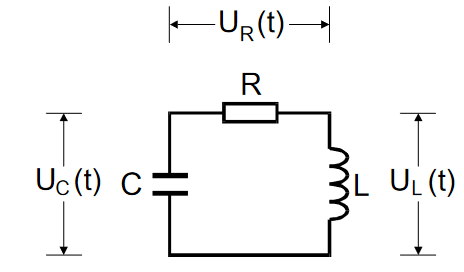
\includegraphics[width=8cm, keepaspectratio]{Schwingkreis}
\caption{Schwingkreis}
\label{fig:Schwingkreis}
\end{figure}
Mit den herkömmlichen Relationen für Kondensator, Spule und Widerstand lassen sich die einzelnen Spannungen durch den Strom $I$ bzw. die Ladung $Q$ ausdrücken. Daraus lässt sich unter Berücksichtigung von
\begin{equation*}
I=\frac{dQ}{dt}
\end{equation*}
die Differentialgleichung für den gedämpften harmonischen Oszillator
\begin{equation}
\frac{d^2I}{dt^2}+\frac{R}{L}\frac{dI}{dt}+\frac{1}{LC}I=0
\end{equation}
herleiten. Diese hat die allgemeine Lösung 
\begin{equation}
I(t)=e^{-2\pi \mu t}(Ae^{2\pi ivt}+Be^{-2\pi ivt})
\end{equation}  
mit der imaginären Einheit $i$ und beliebigen Konstanten $A$ und $B$. Die weiteren Konstanten sind durch 
\begin{equation*}
\mu=\frac{1}{2\pi}\frac{R}{2L}
\end{equation*}
und
\begin{equation}
v=\frac{1}{2\pi}\sqrt{\frac{1}{LC}-\frac{R^2}{4L^2}}
\end{equation}
definiert. Die genaue Form dieser Gleichung hängt nun vom Verhältnis der Größen $\frac{1}{LC}$ und $\frac{R^2}{4L^2}$ zueinander ab. Je nachdem welcher der Terme größer, v also reell oder imaginär, ist ergeben sich drei verschiedene Fälle, für die sich das Verhalten des Schwingkreises qualitativ unterscheidet. \\
Im ersten Fall gilt $1/LC>R^2/4L^2$, v ist also reellwertig. In diesem Fall lässt sich die allgemeine Lösung auf eine Gleichung der Form
\begin{equation*}
I(t)=A_0e^{-2\pi \mu t}cos(2\pi vt+\eta)
\end{equation*}
mit reellen Konstanten $A_0$ und $\eta$ zurückführen. Für diesen Fall zeigt sich also eine gedämpfte Schwingung mit einer e-Funktion als Einhüllenden. Der Wert von $\mu$ bestimmt dabei die Abnahmegeschwindigkeit Schwingung. Der Wert
\begin{figure}
\centering
\includegraphics[width=8cm, keepaspectratio]{gedämpfte Schwingung}
\caption{gedämpfte Schwingung}
\label{fig:gedämpfte Schwingung}
\end{figure}
\begin{equation}
T_{ex}=\frac{2L}{R}
\end{equation}
gibt die Zeitspanne an, nach der die Amplitude das $1/e$-fache seines Ausgangswertes erreicht hat und wird als Abklingzeit bezeichnet. Die Periodendauer der Schwingung beträgt
\begin{equation*}
T=\frac{1}{v}=\frac{2\pi}{\sqrt{1/LC-R^2/4L^2}}
\end{equation*}
\\
Im zweiten Fall ist $1/LC<R^2/4L^2$, v ist also komplexwertig. In diesem Fall besteht die allgemeine Lösung nur noch aus reellen e-funktionen, da die imaginären Anteile durch das imaginäre $v$ kompensiert werden. In diesem Fall zeigt sich eine sogenannte aperiodische Dämpfung, bei welcher kein oszillatorisches Verhalten mehr auftritt. Nach einer gewissen Zeit zeigt sich ein Verlauf der Form 
\begin{equation*}
\exp{-(R/2L-\sqrt{R^2/4L^2-1/LC})t}
\end{equation*}
der einen einfachen Relaxationsvorgang darstellt. \\
Für den dritten Fall $ 1/LC=R^2/4L^2$, also $v=0$, nimmt die allgemeine Lösung die Form
\begin{equation*}
I(t)=Ae^{-\frac{t}{\sqrt{LC}}}
\end{equation*}
an. Dies wird als der aperiodische Grenzfall bezeichnet, bei dem das System schnellstmöglich in seinen Grundzustand zurückkehrt.
\section{Erzwungene Schwingung}
In die vorherige Schaltung wird nun eine Spannungsquelle eingefügt, welche eine sinusförmige Spannung liefert, und dadurch ein System in Form einer angeregten Schwingung erzeugt. Durch die zusätzliche Spannungsquelle nimmt die Differentialgleichung für die Kondensatorspannung in Abhängigkeit von der Zeit die Form
\begin{equation}
LC\frac{d^2U_C(t)}{dt^2}+RC\frac{d^2U_C(t)}{dt^2}+U_C(t)=U_0e^{iwt}
\end{equation}
an. Diese Gleichung hat eine allgemeine Lösung der Form $u(w)e^{iwt}$ mit der komlexen Funktion $u(w)$, für die sich die Gleichung
\begin{equation*}
\frac{U_0(1-LCw^2-iwCR)}{(1-LCw^2)^2+w^2R^2C^2}
\end{equation*}
ergibt wobei sich $U_0$ und $w$ auf Frequenz und Amplitude der anregenden Spannung beziehen. Aus diesem Zusammenhang lassen sich Amplitude und Phase in Abhängigkiet von der Frequenz bestimmen. Die Phasenverschiebung hat die Form
\begin{equation}
\phi(w)=arctan(\frac{-wRC}{1-LCw^2}).
\end{equation}
Aus dem Betrag der Funktion $u(w)$ folgt die Frequenzabhängigkeit der Amplitude, die durch die Gleichung
\begin{equation*}
U(w)=\frac{U_0}{\sqrt{(1-LCw^2)^2+w^2R^2C^2}}
\end{equation*}
beschrieben wird. Hieraus folgt, dass die Amplitude der Kondensatorspannung für verschwindende Frequenzen gegen $U_0$ und für große Frequenzen gegen $0$ geht. Darüber hinaus erreicht die Amplitude bei geeigneter Frequenz ein Maximum, welches signifikant größer als die ursprüngliche Erregerfrequenz ist. Dieses Phänomen wird als Resonanz bezeichnet. Die zugehörige Resonanzfrequenz $w_{Res}$, bei der das Phänomen auftritt, beträgt
\begin{equation}
w_{Res}=\sqrt{\frac{1}{LC}-{R^2}{2L^2}}.
\end{equation}
 Im Falle schwacher Dämpfung, also für einen vernachlässigbar kleinen Widerstand, nähert sich diese Frequenz der Frequenz $w_0$ der ungedämpften harmonischen Schwingung und die Resonanzamplitude beträgt
\begin{equation}
U_{max}=\frac{1}{w_0RC}U_0
\end{equation}
wobei der Faktor $1/w_0RC$ auch als Gütefaktor $q$ bezeichnet wird. Weiterhin von Bedeutung ist die Breite der Resonanzkurve. Diese wird duch die beiden Frequenzen $w_+$ und $w_-$ definiert, an denen die Spannung den Wert $w=1/\sqrt{2}U_0$ annimt. Daraus folgt für die Breite
\begin{equation*}
w_+-w_-\approx \frac{R}{L}.
\end{equation*}
Im umgekehrten Fall der starken Dämpfung , also für $1/LC>>R^2/2L^2$ zeigt das System ein qualitativ anderes Verhalten. Anstelle von Resonanz strebt das System von der Erregerspannung ausgehend gegen $0$. Aufgrund dieser Eigenschaft kann eine solche Schaltung auch als Tiefpass genutzt werden. \\
Da die Phasenverschiebung die Form eines arcustangens hat, verschwindet selbige für$w=0$, während sie sich für sehr hohe Frequenzen dem Wert $\pi$ nähert. Davon Abgesehen kann durch die Gleichung
\begin{equation}
w_{1,2}=\pm \frac{R}{2L}+\sqrt{\frac{R^2}{4L^2}}
\end{equation}
die Frequenz bestimmt werden, an der die Phasenverschiebung den Wert $\pi /4$ bzw. $3\pi/4$ annimt.
